% Chapter Template

\chapter{Option Pricing And Deep Learning} % Main chapter title

\label{Chapter5} % Change X to a consecutive number; for referencing this chapter elsewhere, use \ref{ChapterX}

Deep learning can be applied to option valuation in different ways. The first method is to simulate input parameter, i.e. the market parameters and model parameters and then using a classical method for calculating target values $\bm{y}$ for the given input parameters $\matr{X}$. The method falls within supervised regression where we will use a MLPs network introduced in section \ref{multilayerPerceptron} to approximate the mapping. We will assume for simplicity the stock follow a GBM, hence from earlier chapters the generations of labels for european and american stock options are already presented (Chapter \ref{Chapter2}, \ref{Chapter3}). The theory in chapter \ref{Chapter4} will be specialized for the specific task and discussed. The supervised MLPs regression will be used to valuate european call options and american put options.

%----------------------------------------------------------------------------------------
%	SECTION 1
%----------------------------------------------------------------------------------------

\section{Multilayer Perceptrons Regression For European Options}
For the european option with have a analytical solution to the option pricing problem, hence we can easily produce the data set with input features and target variable $(x,y)$. Remember the 5 parameters for pricing an European put option (proposition \ref{BS-price-EuroCall}). The input data x will be varying combinations of the 5 parameters and the target variable will be generated by the Black-Scholes Euro put price. 

%-----------------------------------
%	SUBSECTION 1
%-----------------------------------
\subsection{Data}

\begin{table}[th]
\caption{Parameter range}
\label{tab:treatments}
\centering
\begin{tabular}{l l l l l l }
\toprule
\textbf{Moneyness} & \textbf{r} & \textbf{$\sigma$} & \textbf{T} \\
\midrule
0.8-1.2 & 1\%-3\% & 0.05-0.5 & 1/252-3.0\\ 
\bottomrule\\
\end{tabular}
\end{table}


\begin{figure}[th]
\centering
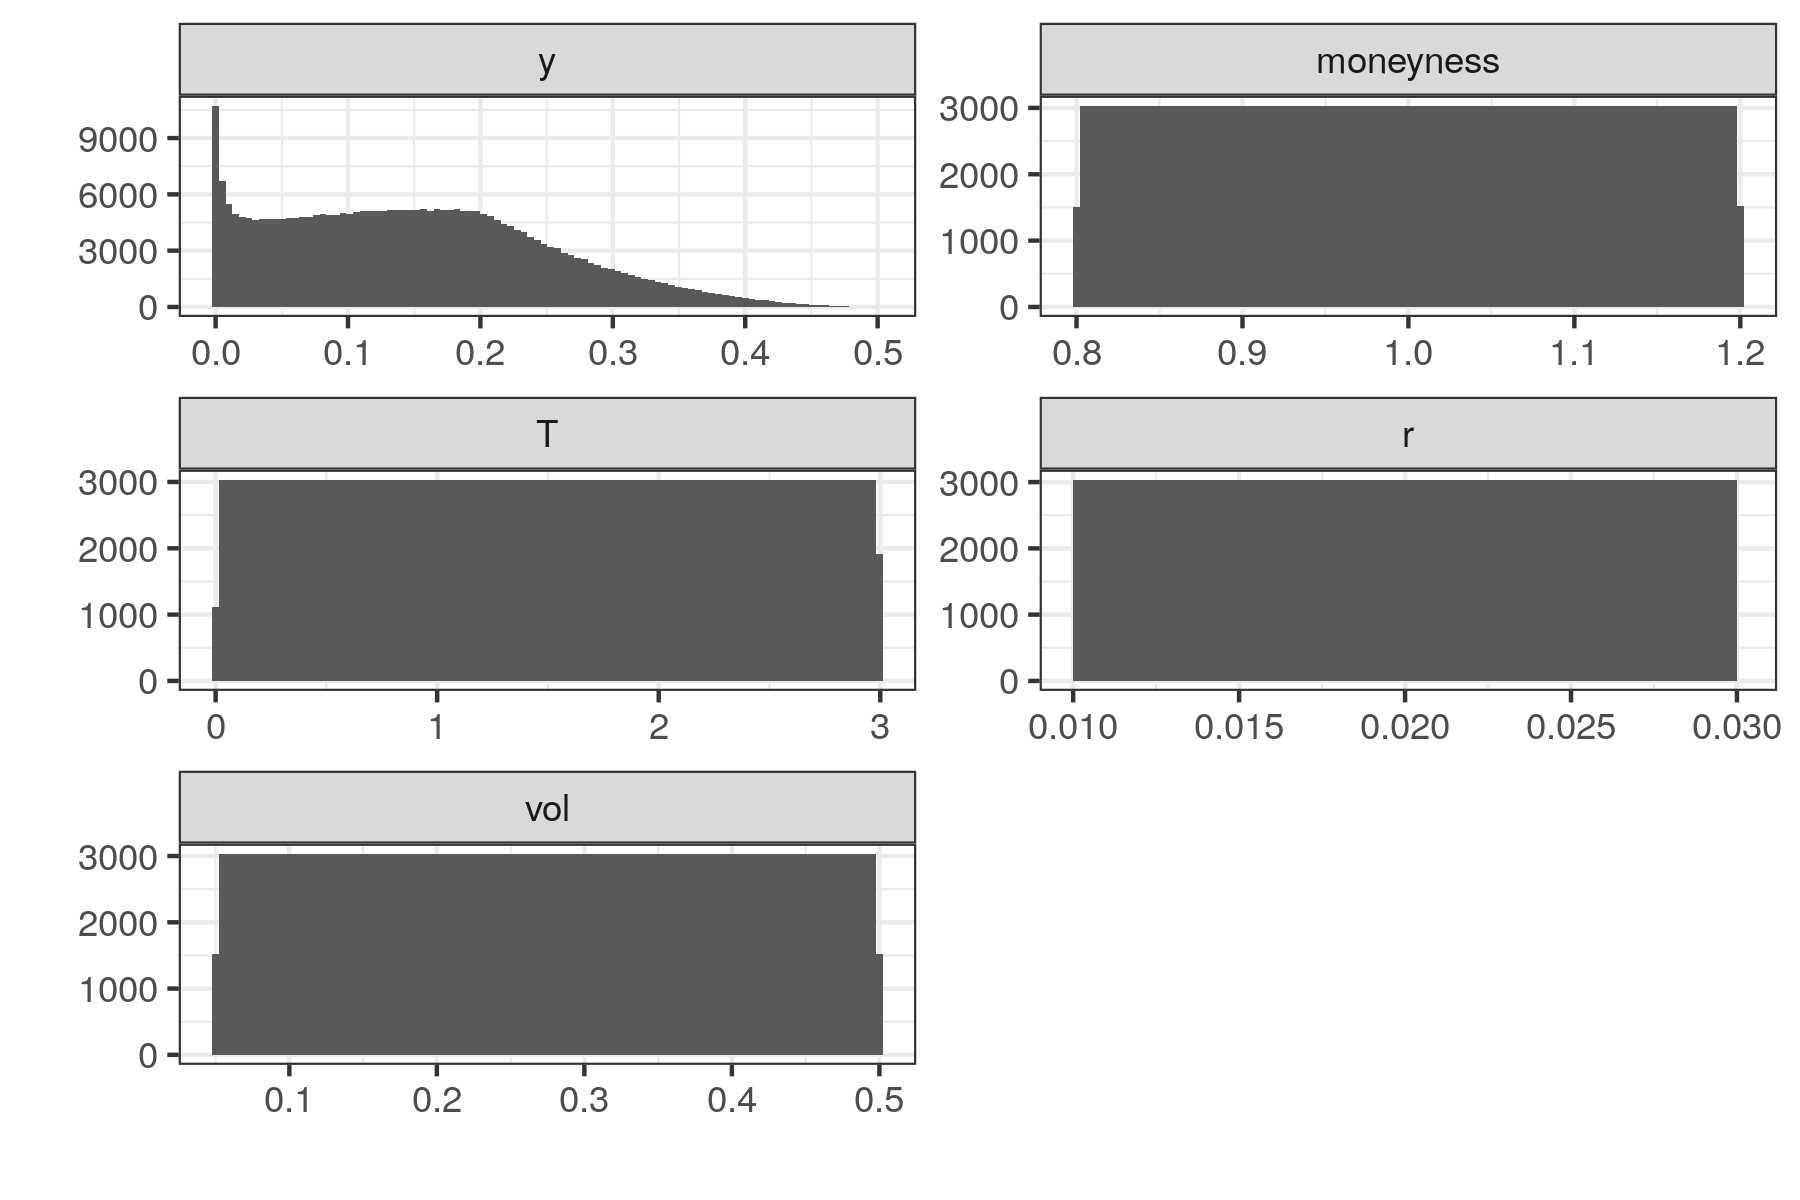
\includegraphics{Figures/marginalEuroCall.png}
\decoRule
\caption[Marginal distributions for european call]{Quasi random simulation with halton sequence}
\label{fig:marginalEuro}
\end{figure}

%-----------------------------------
%	SUBSECTION 2
%-----------------------------------

\subsection{Training}

%-----------------------------------
%	SUBSECTION 3
%-----------------------------------
\subsection{Model Performance}

\begin{figure}[th]
\centering
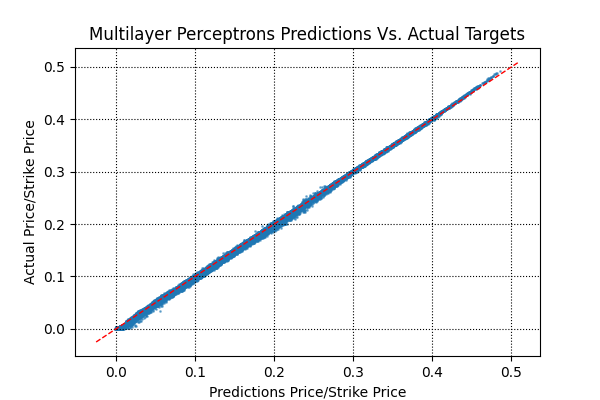
\includegraphics{Figures/PredictionEuroC.png}
\decoRule
\caption[MLPs Predictions Vs. Actual Prices]{Predicted price based on MLPs model}
\label{fig:marginalEuro}
\end{figure}

%----------------------------------------------------------------------------------------
%	SECTION 2
%----------------------------------------------------------------------------------------
\section{Multilayer Perceptrons Regression For American Options}

%-----------------------------------
%	SUBSECTION 1
%-----------------------------------
\subsection{Data}

\begin{figure}[th]
\centering
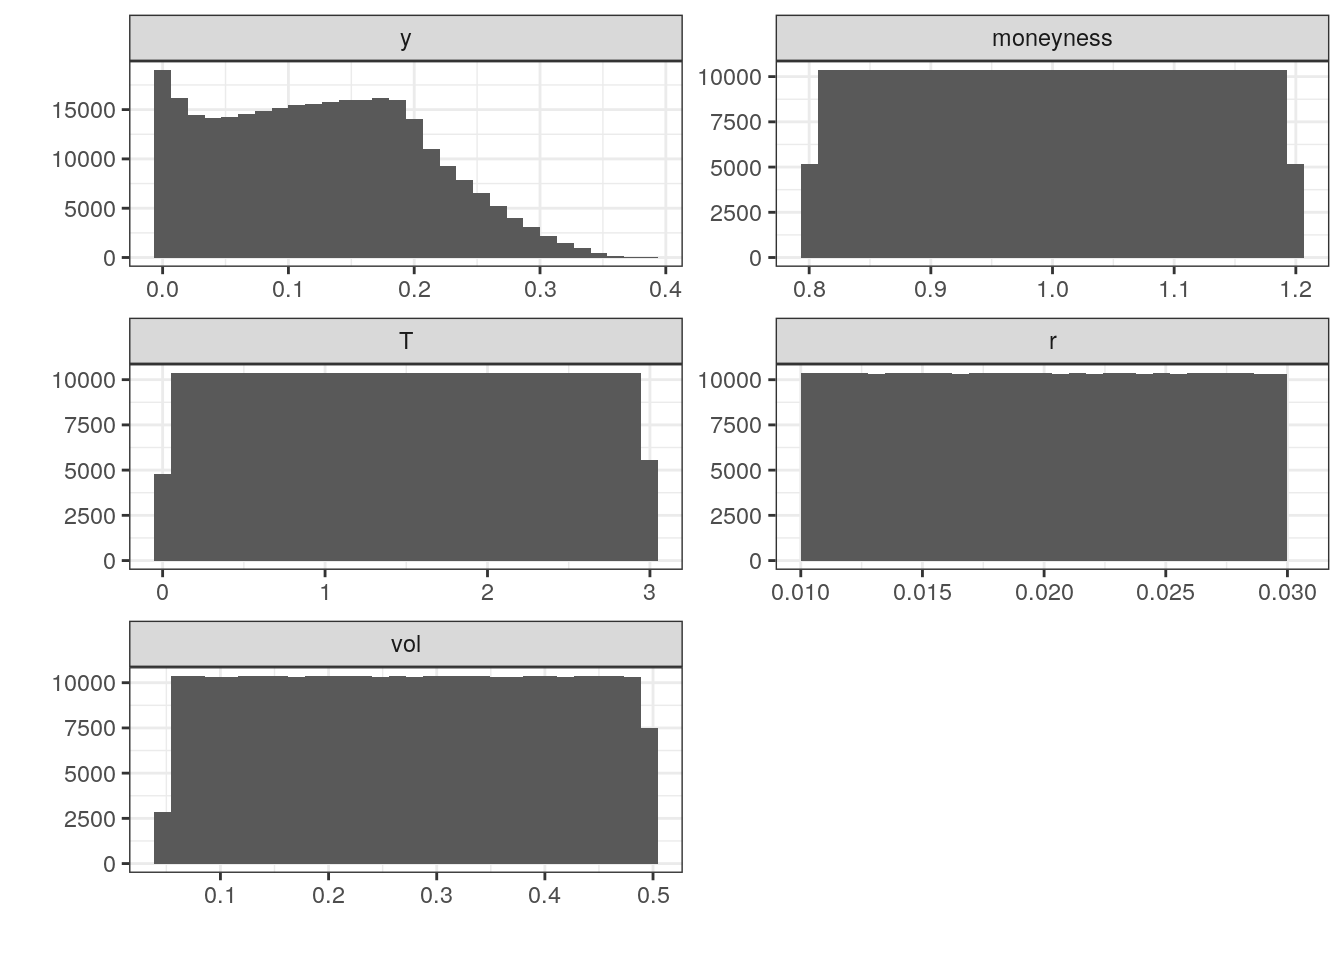
\includegraphics{Figures/marginalAmerPut.png}
\decoRule
\caption[Marginal distributions for american put]{Quasi random simulation with halton sequence}
\label{fig:marginalEuro}
\end{figure}

%-----------------------------------
%	SUBSECTION 2
%-----------------------------------
\subsection{Optimization and cost function}

%-----------------------------------
%	SUBSECTION 3
%-----------------------------------
\subsection{Model Performance}

%------------------------------------------
